\section{Our Code}
    
    \frame{\sectionpage}

{Our code and explanation}
	\begin{verbatim}
	import random
	from flask import Flask
	from flask import request
	from pyspark import SparkConf, SparkContext
	from pyspark.sql import SQLContext, SparkSession
	from pyspark.sql.functions import lower
	
	DEBUG_MODE = False
	IP_ADDR = "0.0.0.0"
	PORT = 80
	
	def init_spark(app_name, master_config):
	"""
	:params app_name: Name of the app
	:params master_config: eg. local[4]
	:returns SparkContext, SQLContext, SparkSession:
	"""
	conf = (SparkConf().setAppName(app_name).setMaster(master_config))
	
	sc = SparkContext(conf=conf)
	sc.setLogLevel("ERROR")
	sql_ctx = SQLContext(sc)
	spark = SparkSession(sc)
	
	return (sc, sql_ctx, spark)
	
	print("### Initializing Spark Context")
	sc, sql_ctx, spark = init_spark("Spark_Webserver", "local[4]")
	print("### Creating Spark dataframe from file")
	df = spark.read.json("quotes-table.json")
	print("### Initializing Flask app")
	#help flask to get resources from the right place
	app = Flask(__name__)
	
	@app.route('/')
	def index():
	# Get author parameter from url
	author_arg = request.args.get('author', default = "", type = str).lower().strip()
	if author_arg == "":
	return '{"error":"Missing author argument","errorcode":0}'
	
	# Get all rows where author column string contains author_arg substring
	author_quotes = df.filter(lower(df.author).like("%" + author_arg + "%"))
	num_quotes = author_quotes.count()
	if num_quotes == 0:
	return '{"error":"Author ' + author_arg + ' has no quotes in table","errorcode":1}'
	
	# Generate random number for row index in author_quotes dataframe table
	random_row = random.randint(0, num_quotes - 1)
	
	# Collect table rows, converting that data to a python list
	rows = author_quotes.collect()
	
	# Retrieve the random row's quote and author
	quote = str(rows[random_row]["quote"])
	author = str(rows[random_row]["author"])
	
	# Return response
	return '{"quote":"' + quote + '", "author":"' + author + '"}'
	
	if __name__ == "__main__":
	print("### Running webserver on", IP_ADDR, "with port", PORT)
	if DEBUG_MODE:
	app.run(host=IP_ADDR, debug=True, port=PORT)
	else:
	from waitress import serve
	serve(app, host=IP_ADDR, port=PORT)
	\end{verbatim}

\begin{frame}{quotes-database}
	\begin{figure}
		\centering
		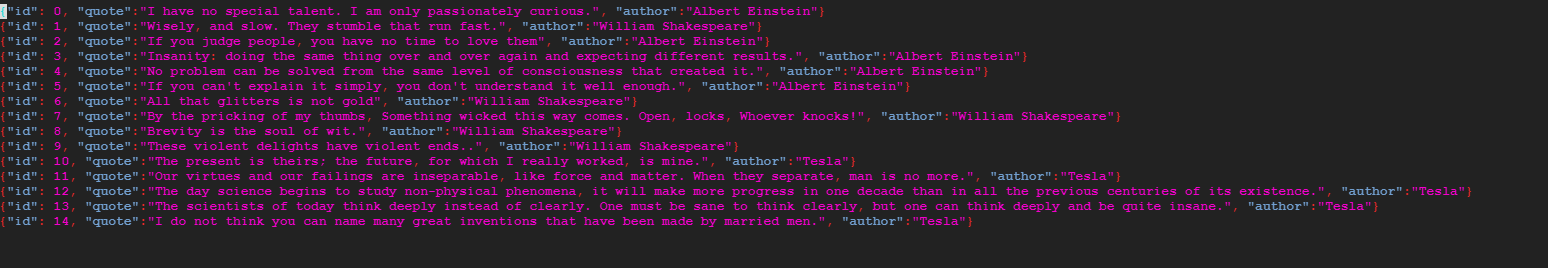
\includegraphics[width =1\linewidth]{robot-spark-proj/quotes-table.PNG}
		\caption{quotes-table}
	\end{figure}
	
\end{frame}

